\chapter{一元函数的微分}
\label{chap:univariate-differentiation}
\label{chap:continuous-functions}

设$f$定义在实轴的区间上。输入从$a$变到$a+h$时，函数值变化了多少？能否把这个变化近似写成$h$的固定倍数？
如果能，一点处的这个倍数又能告诉我们函数在整段区间上的什么行为？本章围绕这三个问题展开。

第一个问题引出导数：用割线斜率的极限描述一点处的变化率，并把它改写为“输入增量乘以一个实系数，再加上相对可忽略的余项”的一次近似。
这里的“乘以一个实系数”在一元情形下已经足够，到线性代数中再统一为线性映射。

随后分别整理四则运算、复合与反函数怎样传递到导数，计算基本函数的导数，并引入高阶导数。

第三个问题由中值定理回答：它把一点处的导数与区间上的增减、凹凸和变化幅度联系起来。
Taylor公式进一步用多项式近似函数，给出可以计算的误差界，并由此把基本函数展开成幂级数、得到Euler公式、分析差分近似的步长。
最后两节分别处理不定式的极限和函数项级数的逐项求导。本章直接使用上一章的极限、连续性与闭区间性质。

\section{导数与微分}
\label{sec:ru-derivatives}
\label{sec:analysis-derivatives-linear-approximation}

设$f$在包含$a$的某个开区间内有定义。输入从$a$变为$a+h$时，函数增量为$\Delta f=f(a+h)-f(a)$。当$h\neq0$时，比值
\[
 \frac{\Delta f}{h}=\frac{f(a+h)-f(a)}h
\]
称为\term{差商}（difference quotient），它是这两个输入之间的平均变化率，在图像上是连接$(a,f(a))$与$(a+h,f(a+h))$的割线斜率。
让$h$趋于零，平均变化率收缩为一点处的变化率。

\begin{definition}[导数]
\label{def:ru-derivative}
若差商在$h\to0$时有有限极限，就称$f$在$a$处可导，并称
\[
 f'(a)=\lim_{h\to0}\frac{f(a+h)-f(a)}h
\]
为$f$在$a$处的\term{导数}（derivative）。若$f$在某个区间内每点可导，$x\mapsto f'(x)$称为导函数。
\end{definition}
某一点的导数是一个数，导函数是一个函数，两者不要混淆。在区间端点，或者在左右变化方式不同的点，可以只让$h>0$或只让$h<0$，分别得到右导数$f'_+(a)$与左导数$f'_-(a)$。
在内点，导数存在当且仅当左右导数都存在且相等；在闭区间的端点讨论导数时，本书总是指从区间内部取得的单侧导数。

直接计算两个例子。对$f(x)=x^2$，差商$[(a+h)^2-a^2]/h=2a+h$，令$h\to0$得$f'(a)=2a$。对$f(x)=|x|$，在原点差商为$|h|/h$：$h>0$时为$1$，$h<0$时为$-1$，
所以$f'_+(0)=1$、$f'_-(0)=-1$，绝对值函数在原点不可导，尽管它在原点连续。
反过来，可导一定连续：$f(a+h)-f(a)=\frac{f(a+h)-f(a)}h\cdot h\to f'(a)\cdot0=0$。所以连续是可导的必要条件，但不充分。
图~\ref{fig:analysis-continuity-counterexamples}比较了平方函数、绝对值函数与阶跃函数在原点的情形。
切线斜率与瞬时变化率都是导数的解释；判断导数是否存在，依据始终是差商的极限，而不是图像上看起来有没有切线。

\begin{figure*}[htbp]
 \centering
 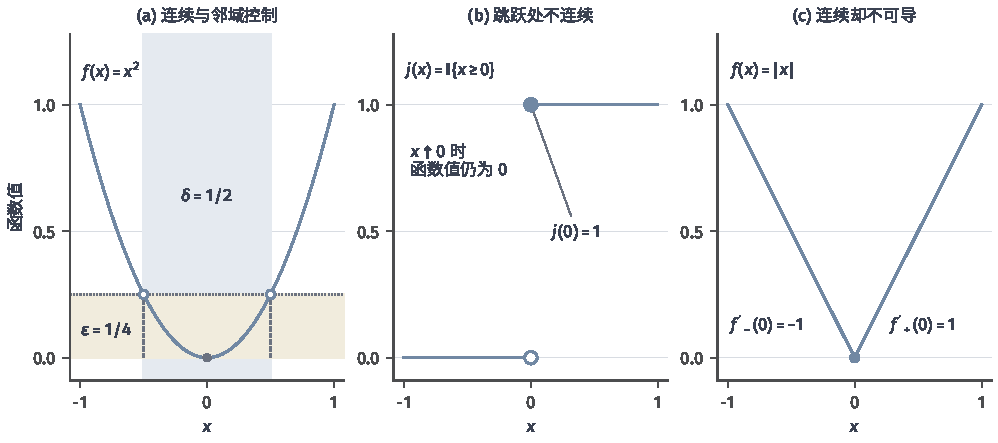
\includegraphics[width=169.0mm]{figures/01-basic-mathematics/02-real-numbers-and-univariate-functions/matplotlib/analysis-continuity-counterexamples/figure.pdf}
 \caption{平方函数、绝对值函数与阶跃函数在原点的差别。平方函数连续且可微；绝对值函数连续，但左右导数不同；阶跃函数的左右极限不同。连续性控制函数值的极限，可微性还要求差商具有同一个有限极限。}
 \label{fig:analysis-continuity-counterexamples}
\end{figure*}

\paragraph{可微与一次近似}
导数的定义可以等价地改写为增量的近似形式。差商趋于$f'(a)$，等价于$[f(a+h)-f(a)-f'(a)h]/h\to0$，即
\begin{equation}
 f(a+h)=f(a)+f'(a)h+o(h),\qquad h\to0.
 \label{eq:analysis-scalar-first-order}
\end{equation}
反过来，若存在实数$A$使$f(a+h)=f(a)+Ah+o(h)$，两边减去$f(a)$、除以$h$再令$h\to0$，可知$f$可导且$A=f'(a)$。
满足这一分解的函数称为在$a$处\term{可微}（differentiable）；对一元函数，可导与可微是同一回事。
这一形式把增量分成两部分：$f'(a)h$是输入增量乘以一个固定系数，称为一次近似；余项相对于$h$可以忽略。
一元情形下，“乘以固定系数”就是最简单的线性关系；多个输入时，这个系数要换成线性映射，留到线性代数部分统一处理。

增量、微分与导数是三个不同的对象。$\Delta f$是实际的函数变化；以$f'(a)$为系数的映射$h\mapsto f'(a)h$称为$f$在$a$处的\term{微分}（differential），常记作$\mathrm df=f'(x)\,\mathrm dx$，其中$\mathrm dx$表示输入增量；
导数$f'(a)$则是这个映射的系数。
\begin{example}[平方函数在$a=3$处的微分]
\label{ex:analysis-square-differential}
设$f(x)=x^2$，$a=3$，则$f'(3)=6$，微分为$6h$。取$h=0.1$，微分给出$0.6$，实际增量为$3.1^2-3^2=0.61$，两者之差$(3+h)^2-9-6h=h^2=0.01$。
\end{example}
一次近似常用来估计误差的传递：测量半径$r$时有误差$\Delta r$，圆面积$\pi r^2$的误差约为$2\pi r\,\Delta r$。
但式~\eqref{eq:analysis-scalar-first-order}中的$o(h)$只说明$h\to0$时余项相对于$h$趋于零，并没有告诉我们在指定的$h=0.1$处余项有多大。
要得到给定步长下可以计算的误差上界，需要后面的中值定理与Taylor公式。
\section{导数的运算规则}
\label{sec:ru-derivative-rules}
\label{sec:analysis-scalar-chain-rules}

直接用定义求导，每个函数都要重新计算差商。若已知几个函数的导数，由它们组合出的函数的导数应能直接算出。
本节在导数已经存在的条件下，分别研究四则运算、复合和取反函数怎样传递到导数，下一节再用这些规则计算基本函数的导数。
以下设$f,g$在所讨论的点$a$的某个开邻域内有定义，并在$a$处可导。

\subsection{导数的四则运算}
\label{sec:ru-derivative-arithmetic}

和的差商等于两个差商之和，常数倍的差商等于差商的同一常数倍，令$h\to0$即得$(f\pm g)'(a)=f'(a)\pm g'(a)$与$(cf)'(a)=cf'(a)$。
乘积的增量可以拆成三部分。记$\Delta f=f(a+h)-f(a)$、$\Delta g=g(a+h)-g(a)$，则
\[
 f(a+h)g(a+h)-f(a)g(a)=g(a)\,\Delta f+f(a)\,\Delta g+\Delta f\,\Delta g.
\]
由一次展开，前两项之和为$[f'(a)g(a)+f(a)g'(a)]h+o(h)$；两个增量都至多与$|h|$同阶，乘积$\Delta f\,\Delta g$与$h^2$同阶，所以也是$o(h)$。读出一次项的系数，得到乘积法则
\begin{equation}
 (fg)'(a)=f'(a)g(a)+f(a)g'(a).
 \label{eq:analysis-scalar-sum-product-rules}
\end{equation}
增量的乘积之所以可以并入余项，是因为两个小量相乘比每个小量都小得多；这一步使乘积的导数只剩两项。

商需要分母非零。设$g(a)\neq0$，可导蕴含连续，所以$g$在$a$附近不为零。先求倒数的导数：
\[
 \frac1h\Bigl(\frac1{g(a+h)}-\frac1{g(a)}\Bigr)=-\frac{g(a+h)-g(a)}h\cdot\frac1{g(a+h)g(a)}\to-\frac{g'(a)}{g(a)^2},
\]
再把$f/g$写成$f\cdot(1/g)$用乘积法则，得到
\[
 \Bigl(\frac fg\Bigr)'(a)=\frac{f'(a)g(a)-f(a)g'(a)}{g(a)^2}.
\]

\subsection{复合函数的求导法则}
\label{sec:ru-chain-rule}

复合函数的输入变化先经过内层、再传入外层，总的一次变化由两层的变化率相乘得到。
\begin{theorem}[链式法则]
\label{thm:ru-chain-rule}
若$f$在$a$处可导，$g$在$f(a)$处可导，且$g\circ f$在$a$的某个邻域内有定义，则
\begin{equation}
 (g\circ f)'(a)=g'(f(a))\,f'(a).
 \label{eq:analysis-scalar-chain-rule}
\end{equation}
\end{theorem}
\begin{proof}
记$b=f(a)$、$k(h)=f(a+h)-f(a)$。由$f$的一次展开，$k(h)=f'(a)h+o(h)$，所以$k(h)\to0$，并且充分小的$h$满足$|k(h)|\leq(|f'(a)|+1)|h|$。
把$g$在$b$处的一次展开写成$g(b+k)=g(b)+g'(b)k+|k|\,\varepsilon(k)$，其中$k\neq0$时$\varepsilon(k)=[g(b+k)-g(b)-g'(b)k]/|k|\to0$，并规定$\varepsilon(0)=0$。代入$k=k(h)$，
\[
 g(f(a+h))-g(f(a))=g'(b)f'(a)h+g'(b)\,o(h)+|k(h)|\,\varepsilon(k(h)).
\]
最后一项的绝对值不超过$(|f'(a)|+1)|h|\,|\varepsilon(k(h))|$，也是$o(h)$。所以一次项系数为$g'(b)f'(a)$。
\end{proof}
证明中规定$\varepsilon(0)=0$，是为了处理内层增量$k(h)$可能为零的情形；若照搬记号$\frac{\mathrm dg}{\mathrm dx}=\frac{\mathrm dg}{\mathrm dy}\cdot\frac{\mathrm dy}{\mathrm dx}$“约去$\mathrm dy$”，就会在$k(h)=0$时除以零。
记号可以帮助记忆，但不能代替证明。用一个能直接展开的例子核对：$(1+x^2)^3$以$y=1+x^2$为中间变量，链式法则给出$3y^2\cdot2x=6x(1+x^2)^2$；
直接展开$(1+x^2)^3=1+3x^2+3x^4+x^6$再求导，得$6x+12x^3+6x^5$，二者相同。

\subsection{反函数的求导法则}
\label{sec:ru-inverse-derivative}

上一章已经证明，区间上连续且严格单调的函数有连续的反函数（定理~\ref{thm:ru-inverse-continuity}）。现在判断反函数何时可导。
设$f$在区间$I$上连续、严格单调，$g=f^{-1}$。设$a$是$I$的内点，$f$在$a$处可导且$f'(a)\neq0$，记$b=f(a)$，$b$是区间$f(I)$的内点。
对充分小的$k\neq0$，令$h=g(b+k)-a$。$g$是单射，所以$h\neq0$；$g$连续，所以$k\to0$时$h\to0$。由$f(a+h)=b+k$，
\[
 \frac{g(b+k)-g(b)}k=\frac h{f(a+h)-f(a)}\to\frac1{f'(a)}.
\]
因此$g$在$b$处可导，且$g'(b)=1/f'(a)$，即$(f^{-1})'(b)=1/f'(f^{-1}(b))$。

对$f(g(y))=y$用链式法则也能得到同一公式，但那要求事先知道$g$可导，所以上面先用差商证明可导性；证明中$h\to0$这一步依赖反函数的连续性。
条件$f'(a)\neq0$不能省略：$x^3$在$0$处导数为零，反函数$\sqrt[3]y$在$0$处的差商为$1/\sqrt[3]{k^2}$，$k\to0$时无界，反函数不可导，图像在原点有一条竖直的切线。
在区间端点只能取单侧差商，结论相应地改为单侧导数。下一节用这一规则求对数与反三角函数的导数。
\section{基本函数的导数}
\label{sec:ru-elementary-derivatives}
\label{sec:analysis-elementary-derivatives}

有了求导规则，复杂函数的求导就归结为少数基本函数。本节先由有限运算和上一章的基本极限得到幂函数、指数和三角函数的导数，
再借反函数与复合的规则得到其余基本函数的导数，并逐项注明成立范围。

常数函数的差商恒为零，恒等函数的差商恒为$1$。对正整数$m$，把$x^m$看成$m$个恒等函数之积，反复使用乘积法则，每一项只对一个因子求导，共$m$项，得$(x^m)'=mx^{m-1}$。
对负整数$m=-n$，在$x\neq0$处由商法则得$(x^{-n})'=-nx^{n-1}/x^{2n}=mx^{m-1}$，形式相同。于是多项式可以逐项求导，例如$(x^3-3x)'=3x^2-3$。

指数函数满足$e^{x+h}=e^xe^h$，由第~\ref{sec:ru-elementary-limits}节的基本极限$(e^h-1)/h\to1$，
\[
 \frac{e^{x+h}-e^x}h=e^x\,\frac{e^h-1}h\to e^x,\qquad\text{即}\ (e^x)'=e^x.
\]
正弦和余弦由加法公式把差商写成两个基本极限的组合：
\[
 \frac{\sin(x+h)-\sin x}h=\sin x\,\frac{\cos h-1}h+\cos x\,\frac{\sin h}h\to\cos x,
\]
同理$(\cos x)'=-\sin x$。这两个推导只用到加法公式和基本极限，不依赖尚未证明的逐项求导；第~\ref{sec:ru-termwise-differentiation}节对指数级数逐项求导会得到同样的结果，可作核对。
由商法则，$(\tan x)'=(\cos^2x+\sin^2x)/\cos^2x=1/\cos^2x=1+\tan^2x$，在$\cos x\neq0$处成立。

其余基本函数是这些函数的反函数或复合。自然对数是指数函数的反函数，指数的导数处处非零，由反函数求导，$(\log x)'=1/e^{\log x}=1/x$（$x>0$）。
反正弦是正弦在$[-\pi/2,\pi/2]$上的反函数。在$(-\pi/2,\pi/2)$内$(\sin)'=\cos>0$，所以对$y\in(-1,1)$，
\[
 (\arcsin y)'=\frac1{\cos(\arcsin y)}=\frac1{\sqrt{1-y^2}},
\]
其中$\cos(\arcsin y)\geq0$保证开方取正号。在$y=\pm1$处，对应的$\cos=0$，反正弦不可导，图像有竖直的切线。
同理$(\arccos y)'=-1/\sqrt{1-y^2}$（$-1<y<1$），而$(\arctan y)'=1/(1+\tan^2(\arctan y))=1/(1+y^2)$对所有实数$y$成立。

一般底数与实数次幂由自然指数和对数定义：$a^x=e^{x\log a}$（$a>0$），$x^\alpha=e^{\alpha\log x}$（$x>0$）。由链式法则，
\[
 (a^x)'=a^x\log a,\qquad (x^\alpha)'=e^{\alpha\log x}\cdot\frac\alpha x=\alpha x^{\alpha-1},\qquad (\log_ax)'=\frac1{x\log a}.
\]
$x^\alpha$的公式只在$x>0$上使用，因为一般实数次幂只对正数定义；$\alpha$为整数时它与前面的结果一致，并且后者在负数处也成立。
表~\ref{tab:analysis-elementary-derivatives}汇总这些公式。把它们与四则运算、链式法则和反函数求导结合，就能求出基本函数经有限次运算与复合得到的函数的导数。

\begin{table}[htbp]
 \centering\small
 \begin{tabular}{@{}lll@{}}
 \toprule
 函数 & 导数 & 成立范围\\
 \midrule
 $x^m$（$m\in\mathbb Z$） & $mx^{m-1}$ & $m\geq0$时$x\in\mathbb R$；$m<0$时$x\neq0$\\
 $x^\alpha$（$\alpha\in\mathbb R$） & $\alpha x^{\alpha-1}$ & $x>0$\\
 $e^x$ & $e^x$ & $x\in\mathbb R$\\
 $a^x$（$a>0$） & $a^x\log a$ & $x\in\mathbb R$\\
 $\log x$ & $1/x$ & $x>0$\\
 $\log_ax$（$a>0$，$a\neq1$） & $1/(x\log a)$ & $x>0$\\
 $\sin x$ & $\cos x$ & $x\in\mathbb R$\\
 $\cos x$ & $-\sin x$ & $x\in\mathbb R$\\
 $\tan x$ & $1/\cos^2x$ & $x\neq\pi/2+k\pi$\\
 $\arcsin x$ & $1/\sqrt{1-x^2}$ & $-1<x<1$\\
 $\arccos x$ & $-1/\sqrt{1-x^2}$ & $-1<x<1$\\
 $\arctan x$ & $1/(1+x^2)$ & $x\in\mathbb R$\\
 \bottomrule
 \end{tabular}
 \caption{基本函数的导数及成立范围。三角函数采用弧度制，$\log$为自然对数。}
 \label{tab:analysis-elementary-derivatives}
\end{table}
\section{高阶导数}
\label{sec:ru-higher-derivatives}

导函数本身也可以求导。若$f'$在某点可导，它在该点的导数称为$f$的二阶导数，记作$f''$；依次定义$f^{(n)}=(f^{(n-1)})'$，约定$f^{(0)}=f$。
例如$f(x)=x^3-3x$时，$f'(x)=3x^2-3$，$f''(x)=6x$，$f'''\equiv6$，四阶及以上导数为零；$e^x$的各阶导数都是$e^x$；$\sin x$的导数按$\cos x,-\sin x,-\cos x,\sin x$四步一循环。

高阶导数存在与高阶导数连续是两个不同的条件。若$f$在开区间$I$上直到$n$阶导数都存在且连续，称$f$为$n$阶\term{连续可微}（continuously differentiable）函数，记作$f\in C^n(I)$；各阶导数都存在时记作$f\in C^\infty(I)$。
多项式、指数和三角函数都属于$C^\infty$。下面的例子说明处处可导的函数，导函数可以不连续。
\begin{example}[处处可导而导函数不连续]
\label{ex:analysis-derivative-not-continuous}
令$f(0)=0$，$x\neq0$时$f(x)=x^2\sin(1/x)$。在原点，差商$h\sin(1/h)$被$\pm|h|$夹住，趋于$0$，所以$f'(0)=0$。在$x\neq0$处，由乘积法则和链式法则，
\[
 f'(x)=2x\sin\frac1x-\cos\frac1x.
\]
取$x_n=1/(2n\pi)\to0$，则$f'(x_n)=-1$，不趋于$f'(0)=0$。所以$f$处处可导，但不属于$C^1(\mathbb R)$，更没有二阶导数$f''(0)$。
\end{example}
导数在原点附近的振荡来自$-\cos(1/x)$一项。可见“$n$阶可导”与“属于$C^n$”需要分别验证；后面的Taylor公式会明确写出用到的是哪一种条件。

乘积的高阶导数有类似二项式定理的公式。对$n$归纳，并用组合数的递推$\binom nk+\binom n{k-1}=\binom{n+1}k$合并同类项，得到Leibniz公式
\[
 (fg)^{(n)}=\sum_{k=0}^n\binom nkf^{(k)}g^{(n-k)},
\]
其中$f,g$在所讨论的点$n$阶可导。例如$(x^2e^x)^{(n)}$中，$x^2$三阶以上的导数为零，只剩三项：
\[
 (x^2e^x)^{(n)}=x^2e^x+n\cdot2x\,e^x+\binom n2\cdot2\,e^x=e^x\bigl(x^2+2nx+n(n-1)\bigr).
\]

复合函数逐层求导时，每次求导都要再用一次链式法则或乘积法则。以第~\ref{sec:ru-function-arithmetic}节的复合函数$g(x)=\sqrt{1-x^2}$为例，在$(-1,1)$上，
\[
 g'(x)=\frac{-2x}{2\sqrt{1-x^2}}=-\frac x{\sqrt{1-x^2}},\qquad
 g''(x)=-\frac{\sqrt{1-x^2}+x^2/\sqrt{1-x^2}}{1-x^2}=-\frac1{(1-x^2)^{3/2}}.
\]
对参数函数族，求导的变量要说清楚：$f_{a,b}(x)=ax+b$关于输入$x$的导数是$a$，二阶导数为$0$；若把$x$固定、改变参数$a$，函数值的变化率则是$x$。
这些逐层计算得到的各阶导数，正是下面Taylor展开所需的系数。
\section{闭区间上可微函数的性质}
\label{sec:ru-interval-differentiable}

导数记录一点处的变化率。本节把它与区间上的极值、净变化、增减方向、弯曲方向以及变化幅度联系起来。
主要对象是在闭区间上连续、在区间内部可微的函数；局部极值与驻点先在内点讨论，各结论分别写明是否需要端点连续、单侧导数或导数的界。

\subsection{局部极值与驻点}
\label{sec:ru-local-extrema}

导数只反映一点附近的变化，与它对应的是只比较邻近函数值的极值。设$c$属于$f$的定义域，若存在$r>0$，使定义域中满足$|x-c|<r$的$x$都有$f(x)\geq f(c)$，
则称$c$为$f$的局部极小点；若其中$x\neq c$的点都满足$f(x)>f(c)$，称为严格局部极小点。不等号反向，得到局部极大点。
局部极值只与附近比较，整个定义域上的最值则与全部输入比较；最小点一定是局部极小点，反之不然。
\begin{theorem}[Fermat定理]
\label{thm:analysis-fermat}
设$c$是区间$I$的内点，$f:I\to\mathbb R$在$c$处可导。若$c$为$f$的局部极小点或局部极大点，则
\begin{equation}
 f'(c)=0.
 \label{eq:analysis-scalar-first-order-necessary}
\end{equation}
\end{theorem}
\begin{proof}
设$c$为局部极小点。充分小的$h\neq0$满足$f(c+h)-f(c)\geq0$，所以$h>0$时差商非负，$h<0$时差商非正。两侧差商趋于同一个导数，于是$f'(c)\geq0$且$f'(c)\leq0$。局部极大点对$-f$论证。
\end{proof}
导数为零的点称为\term{驻点}（stationary point）。Fermat定理说明，内点处可导的局部极值点必为驻点。证明用到了从两侧取差商，所以结论只适用于内点。

在闭区间上找最值时，极值定理保证最值存在，Fermat定理则缩小了候选范围：最值点只可能是端点、内部驻点，或者内部不可导的点。
例如$f(x)=x^3-3x$在$[-2,3]$上，$f'(x)=3(x-1)(x+1)$，驻点为$\pm1$。比较$f(-2)=-2$、$f(-1)=2$、$f(1)=-2$、$f(3)=18$，最大值$18$在端点$3$取得，最小值$-2$在$-2$与$1$两处取得。
导数为零只是内点极值的必要条件。$x^3$在$0$处导数为零，但$x<0$时$x^3<0$、$x>0$时$x^3>0$，$0$不是极值点。
不可导的点也要单独检查：$|x|$在$0$处取最小值，那里没有导数；端点$0$是$x$在$[0,1]$上的最小点，右导数却是$1$。

\subsection{中值定理}
\label{sec:ru-mean-value-theorems}

若函数在区间两端取同一值，整段的净变化为零；在连续、可导的条件下，区间内部必有一点的瞬时变化率也为零。
\begin{theorem}[Rolle定理]
\label{thm:analysis-rolle}
设$a<b$，$f$在$[a,b]$上连续、在$(a,b)$内可导，且$f(a)=f(b)$，则存在$c\in(a,b)$使$f'(c)=0$。
\end{theorem}
\begin{proof}
若$f$为常数，任取$c$即可。否则$f$在某个内点的值不同于$f(a)$。由极值定理，$f$在$[a,b]$上达到最大值和最小值，其中至少有一个与端点值不同，因而在某个内点$c$取得。
$c$是局部极值点，$f$在那里可导，由Fermat定理$f'(c)=0$。
\end{proof}
两端取值不同时，先减去连接两端点的直线，使剩余部分在两端相等，再用Rolle定理。
\begin{theorem}[Lagrange中值定理]
\label{thm:analysis-lagrange-mean-value}
设$a<b$，$f$在$[a,b]$上连续、在$(a,b)$内可导，则存在$c\in(a,b)$使
\begin{equation}
 f(b)-f(a)=f'(c)(b-a).
 \label{eq:analysis-mean-value-theorem}
\end{equation}
\end{theorem}
\begin{proof}
令$H(x)=f(x)-f(a)-\frac{f(b)-f(a)}{b-a}(x-a)$，则$H$满足Rolle定理的条件，且$H(a)=H(b)=0$。由$H'(c)=0$整理即得。
\end{proof}
这就是\term{中值定理}（mean value theorem）的含义：区间上的平均变化率等于某个内点处的瞬时变化率。定理只要求内点可导，不要求导函数连续，也不要求端点的单侧导数存在。
图~\ref{fig:analysis-process-mean-value-parallel}以$f(x)=x^2$、区间$[0,1]$为例：端点割线的斜率为$1$，$c=1/2$处的切线与之平行。

\begin{figure}[!htbp]
 \centering
 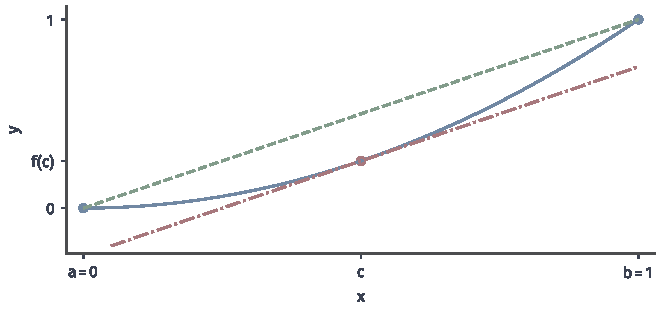
\includegraphics[width=112.0mm]{figures/00-shared/mathematical-preliminaries-upper/00-shared/matplotlib/chapter3-concept-processes/mean-value-parallel.pdf}
 \caption{$f(x)=x^2$在$[0,1]$上，绿虚线为端点割线，红点划线为$c=1/2$处的切线。两线平行，因为$f'(c)=1=[f(1)-f(0)]/(1-0)$。两线高度不同：相等的是斜率，两条直线并不重合。}
 \label{fig:analysis-process-mean-value-parallel}
\end{figure}

比较两个函数在同一区间上的变化时，可以把两者的端点增量放进同一个辅助函数。结论先写成交叉相乘的形式，不需要假设任何分母非零。
\begin{theorem}[Cauchy中值定理]
\label{thm:analysis-cauchy-mean-value}
设$a<b$，$f,g$都在$[a,b]$上连续、在$(a,b)$内可导，则存在$c\in(a,b)$使
\[
 \bigl(f(b)-f(a)\bigr)g'(c)=\bigl(g(b)-g(a)\bigr)f'(c).
\]
若还有$g'(x)\neq0$对每个$x\in(a,b)$成立，则$g(b)\neq g(a)$，并且
\[
 \frac{f(b)-f(a)}{g(b)-g(a)}=\frac{f'(c)}{g'(c)}.
\]
\end{theorem}
\begin{proof}
令$H(x)=(f(b)-f(a))(g(x)-g(a))-(g(b)-g(a))(f(x)-f(a))$，则$H(a)=H(b)=0$，由Rolle定理得$H'(c)=0$，展开即为交叉相乘形式。
若$g'$在内部处处非零，$g(b)=g(a)$会使Rolle定理给出某个内点处$g'=0$，所以$g(b)\neq g(a)$；两边同除以非零的$(g(b)-g(a))g'(c)$即得比值形式。
\end{proof}
取$g(x)=x$即回到Lagrange中值定理。写成比值时要先检查分母：比值形式依赖$g'$在内部处处非零，第~\ref{sec:ru-lhopital}节的L'Hôpital法则正是用这一形式证明的。

\subsection{单调性与凹凸性}
\label{sec:ru-monotonicity-convexity}
\label{sec:analysis-monotonicity}

\paragraph{导数符号与单调性}
中值定理把任意两点之间的增量写成某个内点处的导数乘以输入增量，所以导数的符号可以控制整段的增减。
\begin{theorem}[导数符号与单调性]
\label{thm:analysis-derivative-monotonicity}
设$f$在区间$[a,b]$上连续、在$(a,b)$内可导。若在$(a,b)$内$f'\geq0$，则$f$在$[a,b]$上单调不减；若$f'>0$，则严格递增。$f'\leq0$与$f'<0$相应地给出单调不增与严格递减；若$f'\equiv0$，则$f$为常数。
\end{theorem}
\begin{proof}
任取$a\leq x<y\leq b$，在$[x,y]$上用Lagrange中值定理，$f(y)-f(x)=f'(\xi)(y-x)$，右侧的符号由$f'(\xi)$决定。
\end{proof}
关键是两点之间的整段都属于定义域。在$(0,1)\cup(2,3)$上左段取$0$、右段取$1$的函数导数处处为零，却不是常数，中值定理不能跨过定义域的缺口。
导数处处为正是严格递增的充分条件而非必要条件：$x^3$在$\mathbb R$上严格递增，但在$0$处导数为零。

同样的论证可以判断驻点是否为极值：若$f'$在$c$左侧为负、右侧为正，则$f$在$c$左侧严格递减、右侧严格递增，$c$是严格局部极小点；左正右负则为严格局部极大点。
例如$x^3-3x$的导数$3(x-1)(x+1)$在$1$的左侧为负、右侧为正，$1$是严格局部极小点；在$-1$两侧由正变负，$-1$是严格局部极大点。
若导数在驻点两侧同号，如$x^3$在$0$两侧都有$3x^2>0$，函数沿同一方向变化，驻点就不是极值点。

\paragraph{凸函数}
函数自身的单调性由$f'$的符号决定；$f'$本身的单调性则描述图像的弯曲方向。在区间上任取两点，连接图像上对应两点的线段称为弦。
\begin{definition}[凸函数]
\label{def:ru-convex-function}
设$f$定义在区间$I$上。若对任意$x,y\in I$与$\lambda\in[0,1]$，都有
\[
 f\bigl(\lambda x+(1-\lambda)y\bigr)\leq\lambda f(x)+(1-\lambda)f(y),
\]
即两点之间的图像不高于弦，就称$f$为\term{凸函数}（convex function）；$x\neq y$、$0<\lambda<1$时不等式总是严格成立，称为严格凸函数。若$-f$是凸函数，称$f$为凹函数。
\end{definition}
例如$x^2$是凸函数：$\lambda x^2+(1-\lambda)y^2-(\lambda x+(1-\lambda)y)^2=\lambda(1-\lambda)(x-y)^2\geq0$，并且$x\neq y$时严格大于零。

\begin{theorem}[可微凸函数的刻画]
\label{thm:ru-convexity-derivative}
设$f$在开区间$I$上可微，则下面三条等价：
(1) $f$是凸函数；(2) $f'$在$I$上单调不减；(3) 对任意$x,y\in I$，$f(y)\geq f(x)+f'(x)(y-x)$，即图像总在每条切线的上方。
\end{theorem}
\begin{proof}
(1)$\Rightarrow$(2)：设$x<z<y$，把$z$写成$\lambda x+(1-\lambda)y$，其中$\lambda=(y-z)/(y-x)$，凸性不等式整理后就是三条弦的斜率关系
\[
 \frac{f(z)-f(x)}{z-x}\leq\frac{f(y)-f(x)}{y-x}\leq\frac{f(y)-f(z)}{y-z}.
\]
令$z\to x^+$，左边趋于$f'(x)$；令$z\to y^-$，右边趋于$f'(y)$。所以$f'(x)\leq\frac{f(y)-f(x)}{y-x}\leq f'(y)$。

(2)$\Rightarrow$(3)：由中值定理，$f(y)-f(x)=f'(\xi)(y-x)$，$\xi$在$x,y$之间。$y>x$时$\xi>x$，$f'(\xi)\geq f'(x)$，所以$f(y)-f(x)\geq f'(x)(y-x)$；$y<x$时$f'(\xi)\leq f'(x)$而$y-x<0$，结论相同。

(3)$\Rightarrow$(1)：令$z=\lambda x+(1-\lambda)y$，在$z$处的切线不等式给出$f(x)\geq f(z)+f'(z)(x-z)$与$f(y)\geq f(z)+f'(z)(y-z)$。
两式分别乘以$\lambda$与$1-\lambda$再相加，右侧的一次项因$\lambda(x-z)+(1-\lambda)(y-z)=0$而消去，得到$\lambda f(x)+(1-\lambda)f(y)\geq f(z)$。
\end{proof}
图~\ref{fig:ru-convex-chord-tangent}画出了凸函数与它的一条弦和一条切线：弦在图像上方，切线在图像下方。
凸性要求的是$f'$单调不减，而不是$f$单调：$x^2$在$\mathbb R$上不单调，却是凸函数。

\begin{figure}[!htbp]
 \centering
 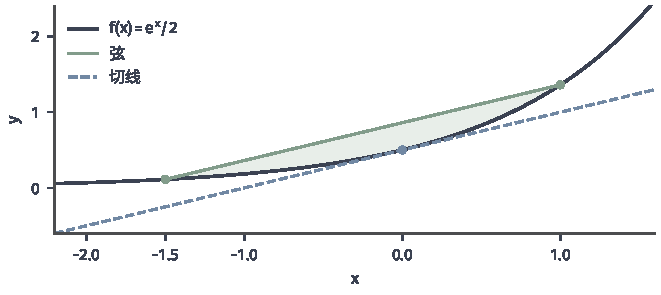
\includegraphics[width=112mm]{figures/01-basic-mathematics/02-real-numbers-and-univariate-functions/matplotlib/convex-chord-tangent/figure.pdf}
 \caption{凸函数$f(x)=e^{x}/2$的弦与切线。绿线连接$x=-1.5$与$x=1$处的两点，两点之间的图像在弦的下方；蓝线是$x=0$处的切线$y=\tfrac12+\tfrac12x$，整条图像在它的上方。图为解析示例。}
 \label{fig:ru-convex-chord-tangent}
\end{figure}

在二阶可微的条件下，凸性可以由二阶导数判断。若$f$在开区间$I$上二阶可导且$f''\geq0$，由定理~\ref{thm:analysis-derivative-monotonicity}，$f'$单调不减，所以$f$是凸函数；
若$f''>0$，则$f'$严格递增，把上面证明中的不等号改为严格，可知$f$严格凸。反方向只对非严格情形成立：凸函数满足$f''\geq0$，因为单调不减的$f'$的导数非负。

严格凸却不要求$f''$处处严格为正。$x^4$的导数$4x^3$在$\mathbb R$上严格递增，所以$x^4$严格凸，但$f''(0)=0$。“二阶导数处处为正”是严格凸的充分条件，不是必要条件。

二阶导数也能判断驻点：若$f'(c)=0$且$f''(c)>0$，则$f'(c+h)/h\to f''(c)>0$，充分小的$h$使$f'(c+h)$与$h$同号，由一阶判别，$c$是严格局部极小点；$f''(c)<0$时是严格局部极大点。
$f''(c)=0$时没有结论：$x^4$、$-x^4$与$x^3$在原点的一、二阶导数都为零，原点分别是极小点、极大点和非极值点。

\paragraph{导数的界}
最后，若导数有统一的界，中值定理把它转化为变化幅度的界。
\begin{theorem}[有界导数与Lipschitz条件]
\label{thm:analysis-bounded-derivative-lipschitz}
设$f$在$[a,b]$上连续、在$(a,b)$内可导，且$|f'(x)|\leq L$对所有$x\in(a,b)$成立，则对任意$x,y\in[a,b]$，$|f(y)-f(x)|\leq L|y-x|$。
\end{theorem}
\begin{proof}
$x\neq y$时，由中值定理$|f(y)-f(x)|=|f'(\xi)|\,|y-x|\leq L|y-x|$。
\end{proof}
例如$\sin$的导数绝对值不超过$1$，所以$|\sin x-\sin y|\leq|x-y|$对所有实数成立。闭区间上的$C^1$函数，导数连续因而有界，于是都是Lipschitz函数。
这说明局部导数信息在具备区间条件时可以给出整体控制。反过来，Lipschitz连续不保证可导：$|x|$在$[-1,1]$上的Lipschitz常数为$1$，在$0$处却不可导。
一元凸性的这些结论将在最优化部分推广到多元函数，并用于判断最优点（\BookChapterRef{chap:optimization}{最优化基础}）。
\section{Taylor公式与局部近似}
\label{sec:ru-taylor}
\label{sec:analysis-taylor-approximation}

一次近似$f(a)+f'(a)h$只用到函数值和斜率，误差是$o(h)$。要提高精度，可以让近似多项式在$a$处与$f$有更多阶相同的导数。
本节先说明这样的多项式怎样确定、误差怎样控制，再把基本函数展开成幂级数并得到Euler公式，最后用同样的工具分析差分近似的误差。

\subsection{Taylor多项式及余项}
\label{sec:ru-taylor-remainders}

设$p(x)=\sum_{k=0}^nc_k(x-a)^k$。逐次求导并代入$x=a$，除了第$k$项外的各项都变为零，得到$p^{(k)}(a)=k!\,c_k$。
所以，要让$p$在$a$处与$f$的前$n$阶导数都相同，系数只能取$c_k=f^{(k)}(a)/k!$。称
\[
 T_n(a+h)=\sum_{k=0}^n\frac{f^{(k)}(a)}{k!}h^k
\]
为$f$在$a$处的$n$阶\term{Taylor多项式}（Taylor polynomial），阶乘来自对$h^k$求$k$次导数。$n=1$时它就是一次近似。

截去的部分$R_n(h)=f(a+h)-T_n(a+h)$称为余项，把函数写成Taylor多项式加余项的等式称为\term{Taylor公式}（Taylor formula）。首先关心的是$h\to0$时余项的阶。
\begin{theorem}[带Peano余项的Taylor公式]
\label{thm:ru-taylor-peano}
设$n\geq1$，$f$在$a$的某个邻域内$n-1$阶可导，且$f^{(n)}(a)$存在，则$h\to0$时
\[
 f(a+h)=\sum_{k=0}^n\frac{f^{(k)}(a)}{k!}h^k+o(h^n).
\]
\end{theorem}
\begin{proof}
对$n$归纳。$n=1$就是可微的定义~\eqref{eq:analysis-scalar-first-order}。设结论对$n-1$成立。$R_n$在$h=0$处为零，它关于$h$的导数$R_n'(h)=f'(a+h)-\sum_{k=1}^n\frac{f^{(k)}(a)}{(k-1)!}h^{k-1}$
恰是$f'$在$a$处的$n-1$阶余项，由归纳假设为$o(h^{n-1})$。由中值定理，$R_n(h)=R_n(h)-R_n(0)=R_n'(\xi)h$，$\xi$在$0$与$h$之间，于是$|R_n(h)|\leq\sup_{|t|\leq|h|}|R_n'(t)|\cdot|h|=o(h^n)$。
\end{proof}
Peano余项只说明误差的阶，不给出指定$h$处的误差大小。若函数在整段上有更高阶的导数，可以把余项写成某个中间点处的导数。
\begin{theorem}[带Lagrange余项的Taylor公式]
\label{thm:analysis-taylor-lagrange}
设$n\geq0$，$h\neq0$，$f$在包含$a$与$a+h$之间闭线段的某个开区间上$n+1$阶可导，则存在严格位于$a$与$a+h$之间的$\xi$，使
\begin{equation}
 f(a+h)=\sum_{k=0}^n\frac{f^{(k)}(a)}{k!}h^k+\frac{f^{(n+1)}(\xi)}{(n+1)!}h^{n+1}.
 \label{eq:analysis-taylor-arbitrary-order}
\end{equation}
若该线段上$|f^{(n+1)}|\leq M$，则$|R_n(h)|\leq M|h|^{n+1}/(n+1)!$。
\end{theorem}
\begin{proof}
记$T(t)=\sum_{k=0}^nf^{(k)}(a)(t-a)^k/k!$，$R=f(a+h)-T(a+h)$，令$H(t)=f(t)-T(t)-R\,(t-a)^{n+1}/h^{n+1}$。
则$H(a+h)=0$，且$H(a)=H'(a)=\cdots=H^{(n)}(a)=0$。先在$a$与$a+h$之间对$H$用Rolle定理得$\xi_1$使$H'(\xi_1)=0$；再在$a$与$\xi_1$之间对$H'$用Rolle定理得$\xi_2$，如此继续。
共用$n+1$次后得到严格位于$a$与$a+h$之间的$\xi$，使$H^{(n+1)}(\xi)=0$。由$T^{(n+1)}=0$，这就是$f^{(n+1)}(\xi)-(n+1)!\,R/h^{n+1}=0$。
\end{proof}
$n=0$时公式就是Lagrange中值定理。误差界说明近似的精度同时取决于阶数、步长和高阶导数的界，三者都可以具体计算。

例如$f(x)=x^3-3x$在$a=1/2$处的二阶Taylor多项式为$T_2=-\tfrac{11}8-\tfrac94h+\tfrac32h^2$，由$f'''\equiv6$，余项恰为$h^3$；取$h=0.1$，$T_2$与真值$-1.584$相差$0.001$。
余项的第三种写法是积分形式，它不含未知的中间点，需要积分，留到第~\ref{sec:ru-integration-by-parts}节推导。

\paragraph{Taylor级数}
有限阶展开、Taylor级数与“函数等于自身的Taylor级数”是三件不同的事。若$f$无穷次可微，可以写出无穷级数$\sum_kf^{(k)}(a)(x-a)^k/k!$，称为$f$在$a$处的Taylor级数；
但这个级数未必收敛到$f$。下面的例子中，Taylor级数在整条实轴上收敛，却只在一点等于原函数。
\begin{example}[光滑但不等于自身Taylor级数的函数]
\label{ex:ru-smooth-not-analytic}
令$f(0)=0$，$x\neq0$时$f(x)=e^{-1/x^2}$。对$x\neq0$归纳可知$f^{(k)}(x)=P_k(1/x)e^{-1/x^2}$，其中$P_k$是多项式。
由$e^u\geq u^m/m!$（$u>0$）取$u=1/x^2$，得$|x|^{-j}e^{-1/x^2}\leq m!\,|x|^{2m-j}$，取$2m>j$即知它在$x\to0$时趋于零。
再在原点用差商逐阶验证，可得$f^{(k)}(0)=0$对每个$k$成立。于是$f$的Taylor级数恒为零，而$x\neq0$时$f(x)>0$。
\end{example}
所以无穷次可微还不足以保证函数能由Taylor级数表示。对具体函数，必须另外证明余项趋于零；下一小节对基本函数逐个完成这一步。

\subsection{基本函数的Taylor展开}
\label{sec:ru-elementary-taylor}
\label{sec:ru-exp-expansion}

本小节把前面的基本函数逐个写成幂级数。这里有两种情形需要分开：$\exp$在第~\ref{sec:ru-elementary-limits}节是\emph{用}级数定义的，级数本身就是定义；
$1/(1-x)$、$\sin x$、$\log(1+x)$等则是事先已有的函数，要\emph{证明}它们等于各自的Taylor级数，并说明在哪些输入上相等。
例如$1/(1-x)$在$x=2$处有值$-1$，它的Taylor级数在那里却发散。

证明的办法都是估计余项$R_n$并证明它趋于零。还要用到一个简单事实：若$m$次以下的多项式$p$满足$f(x)-p(x)=o(x^m)$（$x\to0$），则$p$就是$f$的$m$阶Taylor多项式，因为两个这样的多项式之差也是$o(x^m)$，而非零多项式做不到这一点。

\paragraph{指数函数}
\begin{theorem}[指数函数的展开]
\label{thm:ru-exp-series}
对每个实数$x$，$e^x=\sum_{k=0}^\infty\dfrac{x^k}{k!}$；在$[-A,A]$上，截断到$n$次的误差不超过$e^AA^{n+1}/(n+1)!$。
\end{theorem}
\begin{proof}
由$(e^x)'=e^x$，各阶导数在$0$处都是$1$，Taylor系数为$1/k!$。由Lagrange余项，$|R_n(x)|=e^\xi|x|^{n+1}/(n+1)!\leq e^{|x|}|x|^{n+1}/(n+1)!$，$\xi$在$0$与$x$之间。
右侧是收敛级数$\sum|x|^k/k!$的项，趋于零；$|x|\leq A$时它不超过$e^AA^{n+1}/(n+1)!$。
\end{proof}
这与用级数定义的指数一致：那里级数是定义，这里从导数出发，用余项估计证明函数等于级数，两条路线得到同一个对象。
误差界对整个区间统一成立，例如$A=1$、$n=7$时不超过$e/8!\approx6.7\times10^{-5}$；区间越大，所需阶数越高。
一般底数的指数$a^x=e^{x\log a}$把$x\log a$代入即得$a^x=\sum_k(\log a)^kx^k/k!$。

\paragraph{正弦与余弦}
\begin{theorem}[正弦与余弦的展开]
\label{thm:ru-trig-series}
对每个实数$x$，
\[
 \sin x=\sum_{k=0}^\infty\frac{(-1)^kx^{2k+1}}{(2k+1)!},\qquad\cos x=\sum_{k=0}^\infty\frac{(-1)^kx^{2k}}{(2k)!}.
\]
\end{theorem}
\begin{proof}
正弦和余弦的各阶导数按四步循环，在$0$处的值依次为$\sin$：$0,1,0,-1,\ldots$，$\cos$：$1,0,-1,0,\ldots$，由此得到上面的系数。
各阶导数的绝对值都不超过$1$，Lagrange余项满足$|R_n(x)|\leq|x|^{n+1}/(n+1)!\to0$。
\end{proof}
截断误差可以直接读出：$\sin x\approx x-x^3/6$的四次项为零，用$n=4$的余项得误差不超过$|x|^5/120$。

\paragraph{几何级数}
$f(x)=1/(1-x)$在$0$处的$k$阶导数为$k!$，Taylor系数全为$1$。由有限几何和，余项可以直接写出：
\[
 \frac1{1-x}-\sum_{k=0}^Nx^k=\frac{x^{N+1}}{1-x},
\]
所以$|x|<1$时$1/(1-x)=\sum_{k\geq0}x^k$，$|x|\geq1$时级数发散。

余项公式正好用来观察逼近的质量随输入怎样变化。在$x=0.5$处，取$N=10$误差约为$10^{-3}$；在$x=0.9$处，同样的$N$误差约为$3.1$，要使误差小于$10^{-3}$需要$N\geq87$。
越靠近收敛区间的端点，所需的项数越多，这正是第~\ref{sec:ru-power-series-uniform}节所说的“只在内部闭子区间上一致收敛”。图~\ref{fig:ru-geometric-partial-sums}显示了这一现象。

\begin{figure}[!htbp]
 \centering
 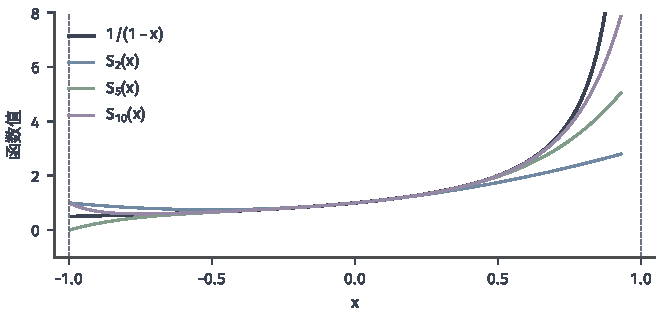
\includegraphics[width=112mm]{figures/01-basic-mathematics/02-real-numbers-and-univariate-functions/matplotlib/geometric-partial-sums/figure.pdf}
 \caption{几何级数的部分和$S_N(x)=\sum_{k=0}^Nx^k$（$N=2,5,10$）与$1/(1-x)$在$(-1,1)$上的比较。中心附近三条曲线几乎重合；越靠近$x=1$，同一个$N$的误差$|x|^{N+1}/|1-x|$越大，在$x=-1$附近部分和则在两侧来回摆动。图为解析示例，纵轴截断在$[-1,8]$。}
 \label{fig:ru-geometric-partial-sums}
\end{figure}

\paragraph{对数与反正切}
这两个函数的导数是有理函数，余项的导数可以写成闭式，于是用中值定理就能估计余项。
\begin{theorem}[对数与反正切的展开]
\label{thm:ru-log-arctan-series}
\[
 \log(1+x)=\sum_{k=1}^\infty\frac{(-1)^{k+1}x^k}{k}\quad(-1<x\leq1),\qquad
 \arctan x=\sum_{k=0}^\infty\frac{(-1)^kx^{2k+1}}{2k+1}\quad(-1\leq x\leq1).
\]
\end{theorem}
\begin{proof}
记$R_n(x)=\log(1+x)-\sum_{k=1}^n(-1)^{k+1}x^k/k$。由有限几何和，
\[
 R_n'(x)=\frac1{1+x}-\sum_{j=0}^{n-1}(-x)^j=\frac{(-x)^n}{1+x}.
\]
$R_n(0)=0$，对$|x|<1$用中值定理，$|R_n(x)|=|R_n'(\xi)|\,|x|\leq|x|^{n+1}/(1-|x|)\to0$。同时$R_n(x)=o(x^n)$，所以这些多项式正是Taylor多项式。

反正切同理：$R_n(x)=\arctan x-\sum_{k=0}^{n-1}(-1)^kx^{2k+1}/(2k+1)$满足$R_n'(x)=(-x^2)^n/(1+x^2)$，于是$|x|<1$时$|R_n(x)|\leq|x|^{2n+1}\to0$。

在端点处，右侧级数由Leibniz判别收敛（对数在$x=1$，反正切在$x=\pm1$）。由Abel第二定理，和函数在包含该端点的闭区间上连续；左侧的函数也连续，两者在端点以内处处相等，所以在端点也相等。
\end{proof}
取$x=1$，得到
\[
 \log2=1-\frac12+\frac13-\cdots,\qquad\frac\pi4=1-\frac13+\frac15-\cdots.
\]
第~\ref{sec:ru-power-series-uniform}节末尾提到的$\sum x^k/k$就是$-\log(1-x)$，它在$x=-1$处的值$-\log2$由此确定。
对数级数在$x=-1$处是调和级数的相反数，发散，与$\log(1+x)\to-\infty$一致。

实数幂$(1+x)^\alpha$也有幂级数展开，即二项式级数，它的证明要用到第~\ref{sec:ru-termwise-differentiation}节的逐项求导，放在那里完成。

\subsection{Euler公式}
\label{sec:ru-euler-formula}
\label{sec:ru-trig-expansion-complex-exponential}

指数级数与正弦、余弦级数只差符号的排列，提示三者有联系。为看清这一点，需要让指数级数接受复数输入。

复数列$z_n\to z$定义为$|z_n-z|\to0$；由$|\operatorname{Re}w|,|\operatorname{Im}w|\leq|w|\leq|\operatorname{Re}w|+|\operatorname{Im}w|$，它等价于实部、虚部分别收敛。
若$\sum|z_k|<\infty$，则实部级数与虚部级数都绝对收敛，因而$\sum z_k$收敛，绝对收敛的结论由此搬到复数。
对每个复数$z$，$\sum|z|^k/k!=e^{|z|}$有限，所以可以定义复指数
\[
 e^z=\sum_{k=0}^\infty\frac{z^k}{k!}.
\]

\begin{theorem}[Euler公式]
\label{thm:ru-euler-formula}
对每个实数$\theta$，$e^{i\theta}=\cos\theta+i\sin\theta$。
\end{theorem}
\begin{proof}
由$i^2=-1$，$i^k$按$1,i,-1,-i$循环，部分和$S_{2N+1}$的偶次项全为实数、奇次项全为虚数：
\[
 S_{2N+1}(i\theta)=\sum_{k=0}^N\frac{(-1)^k\theta^{2k}}{(2k)!}+i\sum_{k=0}^N\frac{(-1)^k\theta^{2k+1}}{(2k+1)!}.
\]
令$N\to\infty$，实部与虚部分别趋于余弦与正弦的展开；整个级数收敛，它的和等于这个子列的极限。
\end{proof}
这里称为\term{Euler公式}（Euler's formula）。证明只把偶次项与奇次项分开读出，没有改变求和次序。

回到复数的三角形式$z=r(\cos\theta+i\sin\theta)$，Euler公式把它写成指数形式$z=re^{i\theta}$：$r$是模，$\theta$是辐角。
第~\ref{sec:ru-complex-geometry}节的“模相乘、辐角相加”变为$r_1e^{i\theta_1}\cdot r_2e^{i\theta_2}=r_1r_2e^{i(\theta_1+\theta_2)}$，整数次幂变为$(re^{i\theta})^n=r^ne^{in\theta}$，三角形式与指数形式由此统一。

特别地，$e^{i\pi}=-1$，$e^{2\pi i}=1$，辐角相差$2\pi$的整数倍正对应$e^{i\theta}$的周期性。本书只使用复数级数，不展开复变函数的微积分。

\subsection{差分近似和步长选择}
\label{sec:ru-finite-differences}

只能计算函数值时，常用差商近似导数。Taylor公式可以说明这种近似的误差有多大。设$f$在$x$附近足够光滑，前向差分的误差由二阶Taylor公式得到：
\[
 \frac{f(x+h)-f(x)}h=f'(x)+\frac{f''(\xi)}2h,
\]
所以$|f''|\leq M_2$时截断误差不超过$M_2h/2$，与$h$同阶。中心差分对称地取两侧，把$f(x\pm h)$各展开到三阶后相减，偶次项抵消：
\[
 \frac{f(x+h)-f(x-h)}{2h}=f'(x)+\frac{f'''(\xi_1)+f'''(\xi_2)}{12}h^2,
\]
$|f'''|\leq M_3$时误差不超过$M_3h^2/6$，与$h^2$同阶，代价是需要三阶导数的界。
用$f(x)=e^x$在$x=0$处核对：取$h=0.1$，前向差分为$(e^{0.1}-1)/0.1\approx1.0517$，误差约$0.052$，接近$h/2=0.05$；中心差分为$(e^{0.1}-e^{-0.1})/0.2\approx1.00167$，误差约$0.00167$，接近$h^2/6\approx0.00167$。

上面的误差分析假定函数值是精确的。实际计算中，函数值本身带有数据误差或舍入误差。设算得的值$\tilde f$满足$|\tilde f-f|\leq\eta$，前向差分的总误差就不超过
\[
 \frac{M_2h}2+\frac{2\eta}h.
\]

第一项是截断误差，随$h$减小而减小；第二项是函数值误差，被除以$h$后放大，随$h$减小而增大。两者之和在$h=2\sqrt{\eta/M_2}$处最小，最小值为$2\sqrt{M_2\eta}$。

以双精度浮点计算为例，$\eta$约为$10^{-16}$乘以函数值的大小，前向差分的合适步长约为$10^{-8}$，而不是越小越好；中心差分的总误差为$M_3h^2/6+\eta/h$，合适步长约为$10^{-5}$\scite{math-nocedal2006numerical}。
图~\ref{fig:ru-finite-difference-error}画出了实际计算的误差：步长大于最优值时，误差沿截断误差的斜率下降；小于最优值后，舍入误差占主导，误差反而上升并剧烈波动。
这里只讨论误差的来源与竞争，系统的数值分析不在本书范围之内。

\begin{figure}[!htbp]
 \centering
 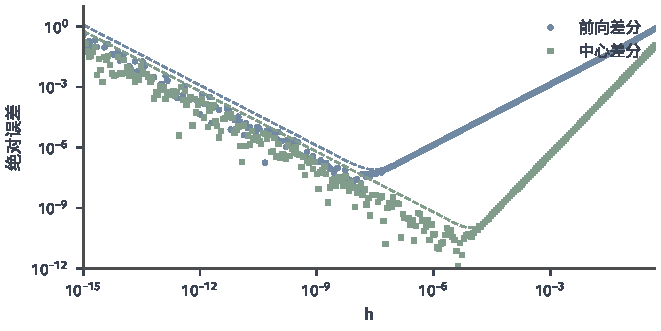
\includegraphics[width=112mm]{figures/01-basic-mathematics/02-real-numbers-and-univariate-functions/matplotlib/finite-difference-error/figure.pdf}
 \caption{用双精度浮点数计算$f(x)=e^x$在$x=1$处导数的差分误差，横轴为步长$h$，两轴均为对数刻度。蓝点为前向差分，绿点为中心差分；虚线是误差模型$eh/2+2\epsilon_{\mathrm{m}}e/h$与$eh^2/6+\epsilon_{\mathrm{m}}e/h$，$\epsilon_{\mathrm{m}}\approx2.2\times10^{-16}$为机器精度。大步长段的斜率分别为$1$与$2$，小步长段的误差随$h$减小而增大。}
 \label{fig:ru-finite-difference-error}
\end{figure}
\section{不定式与L'Hôpital法则}
\label{sec:ru-lhopital}

两个都趋于零的函数相除，比值的极限不能由各自的极限算出，这类形式称为不定式。它问的其实是两个无穷小谁更快趋于零。
函数在趋近点附近可微时，两个函数的增量都可以用导数描述，于是可以借导数比较它们。

\begin{theorem}[L'Hôpital法则]
\label{thm:ru-lhopital}
设$f,g$在$(a,a+r)$内可导，$g'\neq0$，并且$x\to a^+$时$f(x)\to0$、$g(x)\to0$。若$f'(x)/g'(x)\to L$，其中$L$为实数或$\pm\infty$，则$f(x)/g(x)\to L$。左侧与双侧极限有相同的结论。
\end{theorem}
\begin{proof}
补充定义$f(a)=g(a)=0$，则$f,g$在每个$[a,x]$（$x<a+r$）上连续、在内部可导。由Cauchy中值定理的比值形式，存在$\xi_x\in(a,x)$使
\[
 \frac{f(x)}{g(x)}=\frac{f(x)-f(a)}{g(x)-g(a)}=\frac{f'(\xi_x)}{g'(\xi_x)}.
\]
$x\to a^+$时$\xi_x\to a^+$，右侧趋于$L$。比值形式所需的$g(x)\neq g(a)$由$g'\neq0$保证。
\end{proof}
定理中的条件都是充分条件：在趋近点的一侧可导、分母的导数非零、导数比有极限。例如
\[
 \lim_{x\to0}\frac{e^x-1-x}{x^2}=\lim_{x\to0}\frac{e^x-1}{2x}=\frac12,
\]
第二个极限仍是$0/0$型，它由基本极限$(e^x-1)/x\to1$直接得到。法则对$x\to\pm\infty$以及分子分母都趋于无穷的$\infty/\infty$型也成立，证明思路相同\scite{math-lebl-analysis1}。

其他不定式要先转换成$0/0$或$\infty/\infty$，再检查条件。$x\to0^+$时$x\log x$是$0\cdot\infty$型，写成$\log x/(1/x)$后为$\infty/\infty$型，导数比$(1/x)/(-1/x^2)=-x\to0$，所以$x\log x\to0$。
$1^\infty$与$0^0$型先取对数：$(1+1/n)^n=e^{n\log(1+1/n)}$，而$n\log(1+1/n)=\log(1+t)/t$（$t=1/n$）趋于$\log$在$1$处的导数$1$，由指数的连续性，$(1+1/n)^n\to e$。

法则不是万能的，有三点要注意。第一，导数比的极限不存在时，原极限仍可能存在：$x\to+\infty$时$(x+\sin x)/x\to1$，导数比$1+\cos x$却在$0$与$2$之间振荡。
第二，夹逼和等价无穷小比较仍然是独立的工具，很多时候更直接。第三，不能用L'Hôpital法则回头证明$\sin h/h\to1$或$(e^h-1)/h\to1$：
对前者使用法则需要$(\sin)'(0)=1$，而这个导数正是从该极限算出来的，论证会循环。基本极限只能像第~\ref{sec:ru-elementary-limits}节那样用几何或级数直接估计。
\section{函数项级数和幂级数的逐项求导}
\label{sec:ru-termwise-differentiation}

有限和的导数等于各项导数之和。对函数项级数，能否同样逐项求导，就是能否交换“求导”与“取极限”两个操作。
上一章已经看到一致收敛能保持连续性，但下面的例子说明，它不足以保持导数。

令$f_n(x)=\sin(n^2x)/n$。由$|f_n(x)|\leq1/n$，$f_n$在$\mathbb R$上一致收敛到$0$，极限函数的导数为$0$；但$f_n'(x)=n\cos(n^2x)$，在$x=0$处等于$n\to\infty$，并不收敛。
函数值的振幅虽小，振荡的频率却增长得更快，斜率因而越来越大。要交换求导与极限，需要直接控制导数。
\begin{theorem}[函数列的求导与极限交换]
\label{thm:ru-uniform-derivative-limit}
设$f_n$在$[a,b]$上连续可微，导函数列$(f_n')$在$[a,b]$上一致收敛到$g$，并且存在一点$x_0\in[a,b]$使$(f_n(x_0))$收敛。则$f_n$在$[a,b]$上一致收敛到某个可微函数$f$，并且$f'=g$。
\end{theorem}
\begin{proof}
先证$(f_n)$一致收敛。对函数$f_n-f_m$用中值定理，
\[
 |f_n(x)-f_m(x)|\leq|f_n(x_0)-f_m(x_0)|+\sup_{[a,b]}|f_n'-f_m'|\cdot(b-a),
\]
右侧与$x$无关，并且由两个条件可以任意小，由一致柯西准则，$f_n$一致收敛到某个$f$。

再证$f'(c)=g(c)$。对$x\neq c$，记$Q_n(x)=\frac{f_n(x)-f_n(c)}{x-c}$，$Q(x)=\frac{f(x)-f(c)}{x-c}$。对$f_n-f_m$在$c$与$x$之间用中值定理，得$|Q_n(x)-Q_m(x)|\leq\sup|f_n'-f_m'|$，
令$m\to\infty$，由$f_m'$一致收敛到$g$，得$|Q_n(x)-Q(x)|\leq\sup_{[a,b]}|f_n'-g|$，右侧与$x$无关且趋于零，即$Q_n\to Q$对$x$一致。于是
\[
 |Q(x)-g(c)|\leq|Q(x)-Q_n(x)|+|Q_n(x)-f_n'(c)|+|f_n'(c)-g(c)|.
\]
给定$\varepsilon$，先取$n$使第一项和第三项对所有$x$都小于$\varepsilon/3$，再由$f_n'(c)$的定义取$x$足够接近$c$使第二项小于$\varepsilon/3$，所以$Q(x)\to g(c)$。
\end{proof}
证明与上一章连续性保持的论证结构相同：把总误差拆成三段，关键是用一致收敛让同一个$n$对所有$x$有效。这里被一致控制的是差商，它由导数的一致收敛通过中值定理得到。
一点处的收敛条件不能省去：$f_n\equiv n$的导数恒为零，一致收敛到$0$，函数列本身却发散。它排除的正是整列函数一起平移、导数却不变的情形。

\paragraph{函数项级数的逐项求导}
把定理用于部分和$S_N=\sum_{k\leq N}g_k$，就得到逐项求导的条件。
\begin{theorem}[逐项求导]
\label{thm:ru-termwise-derivative}
设各项$g_k$在$[a,b]$上连续可微，导数级数$\sum g_k'$在$[a,b]$上一致收敛，且$\sum g_k(x_0)$在某一点$x_0\in[a,b]$收敛，则$\sum g_k$在$[a,b]$上一致收敛，和函数可微，并且$\bigl(\sum g_k\bigr)'=\sum g_k'$。
\end{theorem}
两个条件各有分工：导数级数的一致收敛控制差商，一点处的收敛确定和函数的取值。

\paragraph{幂级数的逐项求导}
幂级数总满足这些条件，只要停留在收敛区间的内部。
\begin{theorem}[幂级数的逐项求导]
\label{thm:ru-power-series-derivative}
设$\sum c_k(x-x_0)^k$的收敛半径$R>0$，和函数为$S$。则$S$在收敛区间内可微，$S'(x)=\sum_kkc_k(x-x_0)^{k-1}$，且这个导数级数的收敛半径也是$R$。
\end{theorem}
\begin{proof}
由$e^u\geq u^2/2$（取$u=\log k$）得$0\leq(\log k)/k\leq2/\log k\to0$，从而$k^{1/k}=e^{(\log k)/k}\to1$，于是
\[
 \limsup_{k\to\infty}|kc_k|^{1/k}=\limsup_{k\to\infty}|c_k|^{1/k}.
\]
由Cauchy--Hadamard公式，导数级数与原级数有相同的收敛半径（整体乘以$x-x_0$不改变收敛半径）。

导数级数在收敛区间的每个内部闭子区间上一致收敛，原级数在中心收敛，由定理~\ref{thm:ru-termwise-derivative}，在这些闭子区间上可以逐项求导。每一点都落在某个这样的闭子区间中。
\end{proof}
导数级数仍是收敛半径为$R$的幂级数，可以继续逐项求导。于是和函数在收敛区间内无穷次可微，代入$x=x_0$得$S^{(k)}(x_0)=k!\,c_k$：幂级数就是它的和函数的Taylor级数。

例如对$\sum x^k=1/(1-x)$逐项求导，得$\sum_{k\geq1}kx^{k-1}=1/(1-x)^2$（$|x|<1$）；对指数级数逐项求导，又得到$(e^x)'=e^x$，与第~\ref{sec:ru-elementary-derivatives}节由基本极限得到的结果一致。

\paragraph{二项式级数}
逐项求导还能证明实数幂的展开。设$\alpha$为实数，记$\binom\alpha k=\alpha(\alpha-1)\cdots(\alpha-k+1)/k!$（$\binom\alpha0=1$），它们是$(1+x)^\alpha$在$0$处的Taylor系数。
\begin{theorem}[二项式级数]
\label{thm:ru-binomial-series}
对$|x|<1$，$(1+x)^\alpha=\sum_{k=0}^\infty\binom\alpha kx^k$。
\end{theorem}
\begin{proof}
若$\alpha$是非负整数，级数只有有限项，就是二项式定理。否则系数非零，相邻系数之比的绝对值$|\alpha-k|/(k+1)\to1$，收敛半径为$1$。
记和函数为$S$，在$(-1,1)$内逐项求导，并用组合数的关系$(k+1)\binom\alpha{k+1}+k\binom\alpha k=\alpha\binom\alpha k$合并同次项，得到$(1+x)S'(x)=\alpha S(x)$。
于是$g(x)=S(x)(1+x)^{-\alpha}$满足$g'(x)=(1+x)^{-\alpha-1}\bigl[(1+x)S'(x)-\alpha S(x)\bigr]=0$，$g$在$(-1,1)$上为常数$g(0)=1$。
\end{proof}
例如$\alpha=-1$时回到几何级数$1/(1+x)=\sum(-x)^k$，$\alpha=1/2$时$\sqrt{1+x}=1+\tfrac x2-\tfrac{x^2}8+\cdots$。

端点处的求导不能从区间内部的结论自动得到：$\sum x^k/k^2$在$[-1,1]$上收敛，逐项求导得到的$\sum x^{k-1}/k$却在$x=1$处发散。

\FloatBarrier
\section{本章小结}
\label{sec:analysis-summary}

导数把函数增量写成“导数乘以输入增量，再加相对可忽略的余项”。可微蕴含连续，反之不成立；求导规则都由差商的极限或这种一次展开得到，基本函数的导数则回到上一章的两个基本极限。
高阶导数记录变化率本身的变化，Taylor多项式的系数由它们确定。

中值定理把局部信息变成区间上的结论：导数的符号决定单调性，导数的单调性决定凹凸性，导数的界给出Lipschitz界。这些结论都要求所讨论的两点之间整段属于定义域，并在端点连续、内部可微。

Taylor公式控制高阶近似：Peano余项说明误差的阶，Lagrange余项给出有限步长下可计算的误差界；指数、三角、对数等基本函数的余项趋于零，所以它们等于自身的Taylor级数，Euler公式由此得到。
差分近似的截断误差随步长减小，函数值误差却被步长放大，两者的竞争决定了合适的步长。

局部性质、区间保证与极限交换需要分开看待。L'Hôpital法则只是一组充分条件，导数比的极限不存在时原极限仍可能存在；逐项求导要求导数级数一致收敛，函数级数一致收敛还不够。
幂级数在收敛区间内部可以逐项求导，和函数无穷次可微。反过来，已知变化率能否恢复累计量，是下一章积分要回答的问题。
